\chapter{三角比与角边关系}

人们为了要确定空间各点之间的相互位置,就得做一番
测量,测量是几何学的起源,也是几何学最直接的实践。

测量学的最基本原理,就是相似形的性质及三角形的边
角关系。例如,我们在第三章末用相似形性质测量两点间的,
距离,物体的高度、测绘具有多边形形状的地段的平面图
等。我们知道,在两个直角三角形中,只要有一个锐角对应
相等,它们就相似了,这就是说,一个直角三角形的各边之。
间的比是被它的一个锐角的大小所决定,例如在图6.1中,
一些含有$30^{\circ}$角的直角三角形,$30^{\circ}$角所对的直角边与斜边的
比都是1:2.

\begin{figure}[htp]
    \centering
\begin{tikzpicture}
\begin{scope}
\tkzDefPoint(30:2){B_1}
\tkzDefPoints{0/0/A_1, 1.732/0/C_1}
\tkzDrawPolygon(A_1,B_1,C_1)
\tkzMarkAngle[mark=none, size=.5](C_1,A_1,B_1)
\tkzLabelPoints[right](C_1,B_1)
\tkzLabelPoints[left](A_1)
\tkzMarkRightAngle(B_1,C_1,A_1)
\end{scope}
\begin{scope}[xshift=3.5cm]
    \tkzDefPoint(30:3){B_2}
    \tkzDefPoints{0/0/A_2, 2.6/0/C_2}
    \tkzDrawPolygon(A_2,B_2,C_2)
    \tkzMarkAngle[mark=none, size=.5](C_2,A_2,B_2)
    \tkzLabelPoints[right](C_2,B_2)
    \tkzLabelPoints[left](A_2)
    \tkzMarkRightAngle(B_2,C_2,A_2)
\end{scope}
\begin{scope}[xshift=11cm]
    \tkzDefPoint(150:4){B_3}
    \tkzDefPoints{0/0/A_3, -3.464/0/C_3}
    \tkzDrawPolygon(A_3,B_3,C_3)
    \tkzMarkAngle[mark=none, size=.6](B_3,A_3,C_3)
    \tkzLabelPoints[below](C_3,A_3)
    \tkzLabelPoints[left](B_3) 
    \tkzMarkRightAngle(A_3,C_3,B_3)
\end{scope}

\end{tikzpicture}
    \caption{}
\end{figure}

这一章,我们首先向同学介绍的就是直角三角形中,边
与边的比与它所含锐角之间的关系。这些边与边的比值叫做
\textbf{锐角三角比},它们是进行测量计算时的常用数据,也是从数
量方面研究几何学的基本工具。

\section{锐角三角比}

\subsection{定义}

\begin{figure}[htp]\centering
    \begin{minipage}[t]{0.48\textwidth}
    \centering
\begin{tikzpicture}[>=latex, scale=.8]
\draw(30:6)node[right]{$Y$}--(0,0)node[left]{$A$}--(5.5,0)node[right]{$X$};
\draw(30:5)node[above]{$B$}--node[right]{$a$}+(0,-2.5)node[below]{$C$};
\node at (1.25*1.732,0)[below]{$b$};
\node at (30:2.5)[above]{$c$};
\draw(4.33,0) rectangle (4.33-.2,.2);
    \end{tikzpicture}
    \caption{}
    \end{minipage}
    \begin{minipage}[t]{0.48\textwidth}
    \centering
    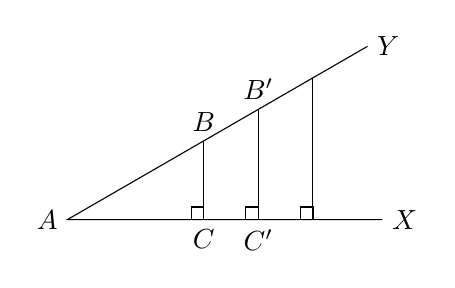
\begin{tikzpicture}[>=latex, scale=.8]
\draw(30:5.5)node[right]{$Y$}--(0,0)node[left]{$A$}--(5,0)node[right]{$X$};
\draw(30:2.5)node[above]{$B$}--+(0,-1.25)node[below]{$C$};
\draw(30:3.5)node[above]{$B'$}--+(0,-1.75)node[below]{$C'$};
\draw(30:4.5)--+(0,-2.25);
\draw(2.165,0) rectangle (2.165-.2,.2);
\draw(3.03,0) rectangle (3.03-.2,.2);
\draw(3.9,0) rectangle (3.9-.2,.2);
    \end{tikzpicture}
    \caption{}
    \end{minipage}
    \end{figure}


取任意锐角$\angle XAY$, 在边$AY$上任取一点$B$, 作$\overline{BC}\bot AX$
于$C$(图6.2). 在直角$\triangle ABC$中,设$\angle A$、$\angle B$、$\angle C$的
对边分别用$a$、$b$、$c$表示,对
锐角$A$来说,$a$叫做$\angle A$的\textbf{对
边},$b$叫做$\angle A$的相邻的直角
边(简称\textbf{邻边})我们定义:
\begin{enumerate}
    \item $\angle A$的对边与斜边的比值,叫做$\angle A$的正弦,用符
号$\sin A$来表示,即
\[\sin A=\frac{\angle A\text{的对边}}{\text{斜边}}=\frac{a}{c}\]
\item $\angle A$的邻边与斜边的比值,叫做$\angle A$的余弦。用符
号$\cos A$来表示,即
\[\cos A=\frac{\angle A\text{的邻边}}{\text{斜边}}=\frac{b}{c}\]
\item $\angle A$的对边与邻边的比值,叫做$\angle A$的正切,用符
号$\tan A$来表示,即
\[\tan A=\frac{\angle A\text{的对边}}{\angle A\text{的邻边}}=\frac{a}{b}\]
\item $\angle A$的邻边与对边的比值,叫做 $\angle A$的余切,用符
号$\cot A$来表示,即
\[\cot A=\frac{\angle A\text{的邻边}}{\angle A\text{的对边}}=\frac{b}{a}\]
\end{enumerate}

我们知道,只要$\angle A$的大
小定了,不管$B$点在边$AY$上
的位置如何(图6.3),以上
的四个比值都是不变的,只有
当$\angle A$变化时,这些比值才随着变化。这四个比都叫做锐角$A$的三角比。

有了以上定义,我们就在直角三角形的角与边之间建立
了联系,知道了角的大小,相应的四个三角比就被唯一地确
定了。反过来,如果我们知道了一个角的四个三角比中的任
何一个,我们也就能确定这个角的大小。

\begin{example}
    在直角$\triangle ABC$中,$\angle C=90^{\circ}$, $\overline{BC}=3$cm, $\overline{AC}=
    4$cm, 求$\angle A$的4个三角比(图6.4)。
\end{example}

\begin{figure}[htp]\centering
    \begin{minipage}[t]{0.48\textwidth}
    \centering
\begin{tikzpicture}[>=latex, scale=1]
\draw(0,0)node[left]{$B$}--node[below]{3}(3,0)node[right]{$C$}--node[right]{4}(3,4)node[above]{$A$}--node[left]{5}(0,0); 
\draw(3,0) rectangle (3-.2,.2);
\draw(3,4-.5) arc (-90:-36.9-90:.5);

    \end{tikzpicture}
    \caption{}
    \end{minipage}
    \begin{minipage}[t]{0.48\textwidth}
    \centering
    \begin{tikzpicture}[>=latex, scale=.8]
\draw(40:7)node[right]{$Y$}--(0,0)node[left]{$A$}--(5,0)node[right]{$X$};
\draw(4.2,0)node[below]{$C$}--node[right]{$1.8$}(4.2,3.56)node[above]{$B$};
\node at (40:3)[left]{$3$};
\node at (2.1,0)[below]{$2.1$};
\draw(4.2,0) rectangle (4,.2);
\draw(.5,0) arc (0:40:.5);
    \end{tikzpicture}
    \caption{}
    \end{minipage}
    \end{figure}

\begin{solution}
    根据勾股定理,
  \[  \overline{AB}=\sqrt{\overline{BC}^2+\overline{AC}^2}=\sqrt{3^2+4^2}=5{\rm (cm)}\]
  根据各三角比的定义有,
\[\begin{split}
    \sin A=\frac{\overline{BC}}{\overline{AB}}=\frac{3}{5},&\qquad \cos A=\frac{\overline{AC}}{\overline{AB}}=\frac{4}{5}\\
    \tan A=\frac{\overline{BC}}{\overline{AC}}=\frac{3}{4},&\qquad \cot A=\frac{\overline{AC}}{\overline{BC}}=\frac{4}{3}\\
\end{split}\]
\end{solution}


\begin{example}
      求$40^{\circ}$角的四个三角比。
\end{example}

\begin{solution}
 用量角器画$\angle XAY=40^{\circ}$(图6.5). 在边$AY$上截
取$\overline{AB}=3$cm(为计算方便,我们尽量取整数),作$\overline{BC}\bot AY$于$C$点,量得$\overline{BC}=1.8$cm, $\overline{AC}=2.1$cm, 在直角
$\triangle ABC$中,根据三角比的定义可得:
\[\sin40^{\circ}=\frac{1.8}{3}\approx 0.6,\qquad \cos40^{\circ}=\frac{2.1}{3}\approx 0.7 \]
\[\tan40^{\circ}=\frac{1.8}{2.1}\approx 0.8,\qquad \cot40^{\circ}=\frac{2.1}{1.8}\approx 1.1\]
\end{solution}

\begin{example}
    已知$\tan A=\frac{1}{2}$, 求$\angle A$.
\end{example}

\begin{figure}[htp]
    \centering
\begin{tikzpicture}
\draw(0,0)node[left]{$A$}--(4,0)node[right]{$C$}--(4,2)node[above]{$B$}--(0,0);
\draw (4,0)rectangle(4-.2,.2);
\end{tikzpicture}
    \caption{}
\end{figure}

\begin{solution}
    作一个直角$\triangle ABC$, 使直角边$\overline{AC}=2$个单位长,
$\overline{CB}=1$个单位长(图6.6),于是,
\[\tan A=\frac{1}{2}\]
用量角器量$\angle A$, 得之$\angle A\approx 26^{\circ}$。
\end{solution}

\begin{ex}
\begin{enumerate}
    \item 已知直角$\triangle ABC$, $\angle C=90^{\circ}$, $\overline{BC}=5$个单位长,$\overline{AC}=
    12$个单位长,求$\angle A$与$\angle B$的四个三角比。
    \item 用作图法求出表中各角的四个三角比的近似值,填入表
    中:
\begin{center}
    \begin{tabular}{c|cccc}
\hline
        $\alpha$ & $20^{\circ}$ & $40^{\circ}$ & $50^{\circ}$ & $80^{\circ}$\\
\hline
$\sin\alpha$\\
$\cos\alpha$\\
$\tan\alpha$\\
$\cot\alpha$\\
\hline
    \end{tabular}
\end{center}
\item 已知 $\sin\alpha=\frac{3}{4}$,
用作图法求$\angle\alpha$.
\item 已知$\cos\beta=\frac{2}{5}$,
用作图法求$\angle \beta$.
\item 已知$\tan A=\frac{3}{5}$, 
用作图法求$\angle A$.
\end{enumerate}
\end{ex}

\subsection{$0^{\circ}$到$90^{\circ}$角的三角比的变化}
半径等于1个单位长的圆叫做\textbf{单位圆}。下面我们利用单
位圆来研究锐角三角比的变化规律:

\begin{figure}[htp]
    \centering
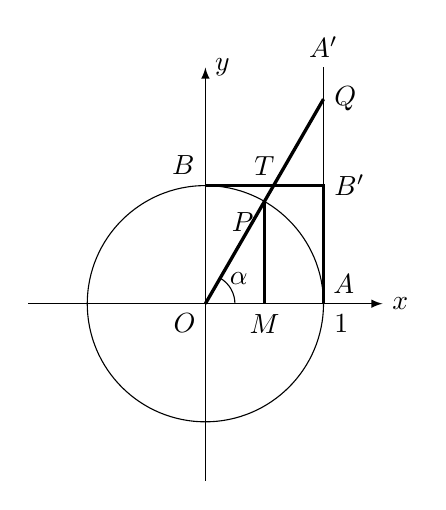
\begin{tikzpicture}[>=latex,scale=1.5]
\draw[->](-1.5,0)--(1.5,0)node[right]{$x$};
\draw[->](0,-1.5)--(0,2)node[right]{$y$};    

\draw(0,0)node[below left]{$O$} circle (1);
\draw(1,0)node[above right]{$A$}--(1,2)node[above]{$A'$};
\draw[very thick](0,0)--(60:1)node[below left]{$P$}--(60:2)node[right]{$Q$};
\draw[very thick](60:1)--(0.5,0)node[below]{$M$};
\draw[very thick](0,1)node[above left]{$B$}--(1,1)node[right]{$B'$}--(1,0)node[below right]{1};
\node at (.5,1)[above]{$T$};
\draw (.25,0) arc (0:60:.25)node[right]{$\alpha$};
\end{tikzpicture}
    \caption{}
\end{figure}


画单位圆$\odot O$(图6.7), 通过单位圆的圆心$O$作互相
垂直的两条直线,其中一条是
水平的,另一条是铅直的,以
$O$为原点,单位圆的半径为长
度单位,在两条直线上建立数
轴,其中水平轴向右为正,铅
直轴向上为正;水平轴用$x$表
示,又叫做$x$轴,铅直的轴用
$y$表示,又叫做$y$轴。以$O$为
顶点,$x$轴的正方向为一边,作$\angle AOP$等于已知角$\alpha$, $\angle AOP$
的两边分别与单位圆相交于$A$、$P$两点,过$P$点作$\overline{PM}\bot OA$于$M$点,

$\because\quad \overline{OP}=1$

$\therefore\quad \sin\alpha=\frac{\overline{MP}}{\overline{OP}}=\overline{MP}\text{的量数},\quad \cos\alpha=\frac{\overline{OM}}{\overline{OP}}=\overline{OM}\text{的量数}$

这样,对于任一锐角$\alpha$, 我们可直接用$\overline{MP}$和$\overline{OM}$的量
数来分别表示$\sin\alpha$, $\cos\alpha$的值。我们把$\overline{MP}$和$\overline{OM}$分别叫做
角$\alpha$的\textbf{正弦线}和\textbf{余弦线}。下面我们用正弦线和余弦线来研究
$\sin\alpha$与$\cos\alpha$的变化规律。




























